\documentclass[12pt,modern]{article}
\usepackage{setspace}
\usepackage{siunitx}
\usepackage{graphicx}
\usepackage[margin=1in]{geometry}

\doublespacing
% \pagestyle{fancy}
% \fancyhf{}
% \lhead{AU Mic Research Overview}
% \rhead{Cail Daley}

\author{Cail Daley}
\title{On the Relation Between Intrinsic and RV-Traced Exoplanet Distributions}

\begin{document}
\maketitle

The true exoplanet distribution across a given parameter (planet mass, semi-major axis, etc.)  is not, of course, perfectly traced by the distribution derived from radial velocity observations. 
This is due to a variety of factors and biases, e.g. the bias towards high-mass planets close to their host star. 
Assuming we can accurately characterize these biases, it should be possible to find the “true” exoplanet distribution that corresponds to the distribution traced by RV techniques. 
While such a goal falls outsides the scope of this project, I would like to take inspiration from this concept and explore the relations between intrinsic distributions and those traced by RV techniques. 
This will be a primarily computational project, comprised of at least three major components: (i) creation of exoplanet distributions (ii) creation of an `observed' light curve for each planetary system in a distribution as part of a hypothetical RV survey, and (iii) fitting the lightcurve with MCMC (and possibly nested sampling) techniques. 
Each component is discussed in a section below.
As this project is still in its infancy in terms of implementation, I give a short description of my (planned) methodology and then mention some of the problems and questions I've been wrestling with in bullet points. I welcome all commentary, but the bullet points are the things I especially need help on.

\section{Creation of an Exoplanet Distribution}
\label{sec: (1)}
A distribution is made up of a set planetary systems; each system is defined by an inclination and a stellar mass. 
I ignore spectral type, stellar metallicity, and distance to the star (these are the ones I can think of; there's probably more). 
Spectral type and stellar metallicity seem beyond the scope of this project as there are no simple theoretical relations that I know of between these two qualities and the RV noise/sensitivity. 
A variable number of planets are added to each system; each planet is defined by a mass, semi-major axis, eccentricity, argument of periastron $\omega$, and time since periastron $t_0$.

\begin{enumerate}
  \item As discussed in Section \ref{sec: (2)}, the stellar distance clearly limits the minimum semiamplitude $K_1$ that can be detected. What do you think I lose by not taking distance into account, or equivalently, setting all systems to the same (undefined) distance? Are there biases that get `washed out' by doing this?
  \item Should I create a uniform distribution (for example, with the same number of Jupiter-mass planets as Mars-mass planets, or the same number of 50 au planets as 0.5 au planets), or should I try to make the distribution look like our own universe's so that we can directly learn about our own exoplanet distribution?
  The former only allows relative comparisons between the true and observed distributions, and would be pretty simple to set up. The latter would be much trickier and prone to error, but could lead to some more interesting results.. what do you think?
\end{enumerate}

\section{Creating a Lightcurve}
\label{sec: (2)}

I create synthetic radial velocity curves using the system and planet properties described in Section \ref{sec: (1)}; an example can be found in Figure \ref{fig: sample}. 
This involves solving Kepler's equation for a set of observation timestamps, etc. etc. 
The resulting resulting curves agree well with theoretical predictions; for a $e=0$ Jupiter analogue around a solar analogue, I derive a $K_1$ of \SI{28.42}{m/s}, compared to the theoretical value of \SI{28.43}{m/s}.  

\begin{figure}
  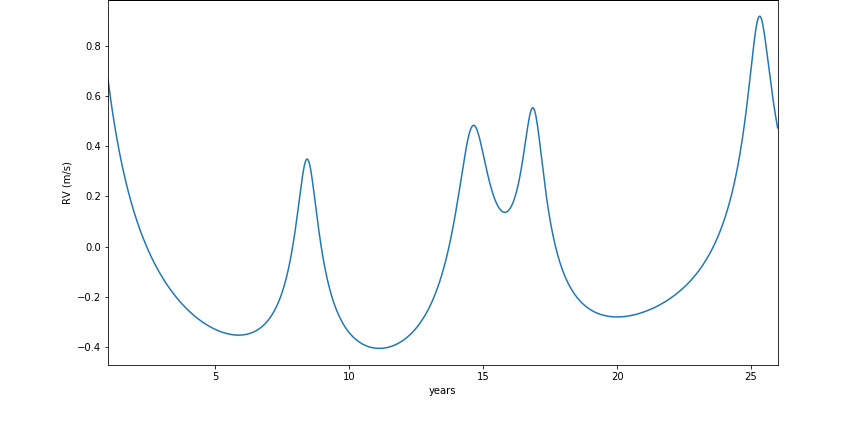
\includegraphics[width=\linewidth]{sample_curve}
  \caption{Analytic RV curve of a four-planet system, with planet parameters listed at the top of the figure. The star is a solar analogue.}
  \label{fig: sample}
\end{figure}

One of the key decisions here is how to determine the periods between radial velocity `observations.' The observations can't be scheduled using any a priori knowledge of the system (that's cheating!), but at the same time observations must be taken such that very short-period planets aren't missed. Additionally, I can't have too many data points; not only is this unrealistic, but it will make the MCMC fitting extremely expensive (see Section \ref{sec: (3)}). Seth suggested that I/the survey `take' two data points separated by a day or so; without doing any modeling, I can use difference between the radial velocity values to decide how to space observations. If there's a big jump in the RV value, I might want to come back the next night, but if it barely changes at all I might wait several months. This seems like a good way to do it, but it's rather contrived, so I'd love to here alternatives!

Noise is added to the analytic RV curve to make the data more realistic (Figure \ref{fig: noisy_sample}); at the moment I'm thinking about adding a constant Gaussian noise of width $\sigma$ somewhere between 1 and \SI{5}{km/s}, but this might not be sufficient. Noise (as well as time between observations) is the only thing stopping the MCMC modeling from finding the correct solution every time; as such, it's super important that I make it realistic. Seth suggested adding (quasi)periodic noise to simulate stellar activity cycles, but this may once again be a little too ambitious..

\begin{figure}
  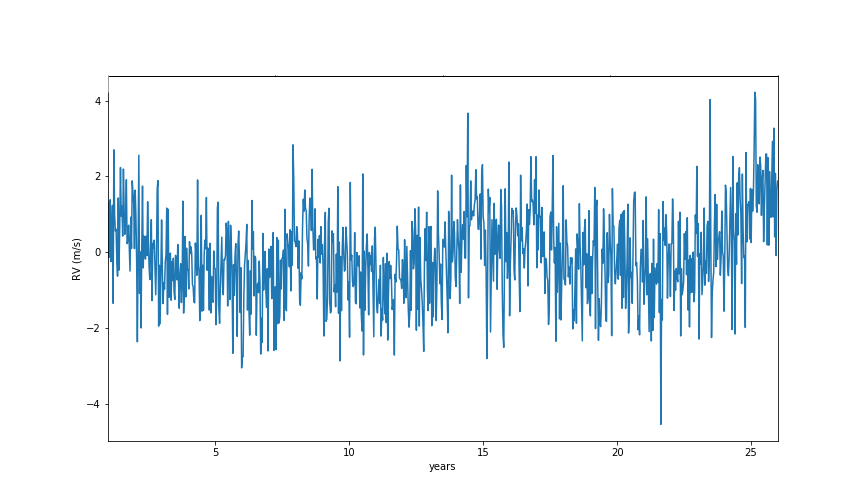
\includegraphics[width=\linewidth]{sample_curve_noisy}
  \caption{Same as Figure \ref{fig: sample}, but with \SI{1}{m/s} Gaussian noise added.}
  \label{fig: noisy_sample}
\end{figure}


\begin{enumerate}
  \item How should I determine the observation time steps?
  \item How should I characterize the noise?
\end{enumerate}


\section{Fitting the Lightcurve}
\label{sec: (3)}

For each system, I will use MCMC methods and maybe nested sampling to fit the `observed' lightcurve. 
Because there will be an unknown number of planets in the system, I will probably have to try several different model formalisms, each with a different number of planets. 
The $\chi^2$ values of models with different numbers of free parameters are not directly comparable, but I can use the Aikake Information Criterion (AIC) to determine relative goodness of fit. 
The AIC basically penalizes you for adding free parameters, since it's almost always possible to get a better fit by using a more complex model. 
I think the most (computationally) efficient way to determine the number of planets is to start with a one-planet fit, and then see if a two-planet fit does better, and repeat until a $n$ planet fit does worse than an $n-1$ planet fit. Once this is the case I call it a day for that particular system, and save the best fit model from the most likely model formalism.

\begin{enumerate}
  \item When determining the number of planets that best fits a system with more than $n$ planets, my algorithm would fail if the relative likelihood of an $n$ planet fit is lower than an $n+1$ planet fit. Is this possible? Is there ever a situation where $n$ planets fits worse than $n+1$ planets, assuming there really are at least $n+1$ planets in the system?
\end{enumerate}


\section{Comparing the Distributions}
\label{sec: (4)}
Once all the systems in a distribution have been fit, we can compare the `true' exoplanet distribution to the distribution constructed from the best fit model parameters from each system. While it will be difficult to make statements about our particular exoplanet distribution, it should be possible to make general statements about the regions of exoplanet parameter space that RV observations are sensitive to.

\begin{enumerate}
  \item Once I have the two distributions, what other cool analyses could I do?
\end{enumerate}

\end{document}
